\documentclass[11pt,openany]{article}

\usepackage{mathtools, commath}
% Packages for formatting
\usepackage[margin=1in]{geometry}
\usepackage{fancyhdr}
\usepackage{enumerate}
\usepackage{graphicx}
\usepackage{kotex}
\usepackage{arydshln} % Include this package
\usepackage{bbding}
\usepackage{amsmath}
\usepackage{amsthm}
\usepackage[dvipsnames,table]{xcolor}
\usepackage{amssymb, amsfonts}
\usepackage{wasysym}
\usepackage{footnote}
\usepackage{tablefootnote}
\usepackage{arydshln} % Include this package
% Fonts
\usepackage[T1]{fontenc}
\usepackage[utf8]{inputenc}
\usepackage{newpxtext,newpxmath}
\usepackage{sectsty}

% Define colors
\definecolor{TealBlue1}{HTML}{0077c2}
\definecolor{TealBlue2}{HTML}{00a5e6}
\definecolor{TealBlue3}{HTML}{b3e0ff}
\definecolor{TealBlue4}{HTML}{00293c}
\definecolor{TealBlue5}{HTML}{e6f7ff}

\definecolor{thmcolor}{RGB}{231, 76, 60}
\definecolor{defcolor}{RGB}{52, 152, 219}
\definecolor{lemcolor}{RGB}{155, 89, 182}
\definecolor{corcolor}{RGB}{46, 204, 113}
\definecolor{procolor}{RGB}{241, 196, 15}

\usepackage{color,soul}
\usepackage{soul}
\newcommand{\mathcolorbox}[2]{\colorbox{#1}{$\displaystyle #2$}}
\usepackage{cancel}
\newcommand\crossout[3][black]{\renewcommand\CancelColor{\color{#1}}\cancelto{#2}{#3}}
\newcommand\ncrossout[2][black]{\renewcommand\CancelColor{\color{#1}}\cancel{#2}}

\usepackage{hyperref}
\usepackage{booktabs}

% Chapter formatting
\definecolor{titleTealBlue}{RGB}{0,53,128}
\usepackage{titlesec}
\titleformat{\section}
{\normalfont\sffamily\Large\bfseries\color{titleTealBlue!100!gray}}{\thesection}{1em}{}
\titleformat{\subsection}
{\normalfont\sffamily\large\bfseries\color{titleTealBlue!50!gray}}{\thesubsection}{1em}{}

%Tcolorbox
\usepackage[most]{tcolorbox}
\usepackage{multirow}
\usepackage{multicol}
\usepackage{blindtext}

\usepackage[linesnumbered,ruled]{algorithm2e}
\usepackage{algpseudocode}
\usepackage{setspace}
\SetKwComment{Comment}{/* }{ */}
\SetKwProg{Fn}{Function}{:}{end}
\SetKw{End}{end}
\SetKw{DownTo}{downto}

% Define a new environment for algorithms without line numbers
\newenvironment{algorithm2}[1][]{
	% Save the current state of the algorithm counter
	\newcounter{tempCounter}
	\setcounter{tempCounter}{\value{algocf}}
	% redefine the algorithm numbering (remove prefix)
	\renewcommand{\thealgocf}{}
	\begin{algorithm}
	}{
	\end{algorithm}
	% Restore the algorithm counter state
	\setcounter{algocf}{\value{tempCounter}}
}

\usepackage{adjustbox}
% Header and footer formatting
\pagestyle{fancy}
\fancyhead{}
\fancyhf{}
\rhead{\textcolor{TealBlue2}{\large\textbf{Linear Algebra \& Abstract Algebra}}}%\rule{3cm}{0.4pt}}
%\chead{\textcolor{TealBlue}{\large\it Think Globally, Act Locally}}
\lhead{\textcolor{TealBlue2}{\large\textbf{[Summer 2025] Mathematics Seminar}}}
% Define footer
%\newcommand{\footer}[1]{
%\begin{flushright}
%	\vspace{2em}
%	\includegraphics[width=2.5cm]{school_logo.jpg} \\
%	\vspace{1em}
%	\textcolor{TealBlue2}{\small\textbf{#1}}
%\end{flushright}
%}
%\rfoot{\large Department of Information Security, Cryptogrphy and Mathematics, Kookmin Uni.\includegraphics[height=1.5cm]{school_logo.jpg}}
\fancyfoot[L]{\large\it \textcolor{TealBlue}{\bfseries Think Globally, Act Locally}}
\fancyfoot[C]{-\thepage-}

\usepackage{tcolorbox}
\tcbset{colback=white, arc=5pt}

\definecolor{axiomcolor}{HTML}{a88bfa}
\definecolor{defcolor}{RGB}{52, 152, 219}
\definecolor{procolor}{RGB}{241, 196, 15}
\definecolor{thmcolor}{RGB}{231, 76, 60}
\definecolor{lemcolor}{RGB}{155, 89, 182}
\definecolor{corcolor}{RGB}{46, 204, 113}
\definecolor{execolor}{RGB}{90, 128, 127}

% Define a new command for the custom tcolorbox
\newcommand{\axiombox}[2][]{%
	\begin{tcolorbox}[colframe=axiomcolor, title={\color{white}\bfseries #1}]
		#2
	\end{tcolorbox}
}

\newcommand{\defbox}[2][]{%
	\begin{tcolorbox}[colframe=defcolor, title={\color{white}\bfseries #1}]
		#2
	\end{tcolorbox}
}

\newcommand{\lembox}[2][]{%
	\begin{tcolorbox}[colframe=lemcolor, title={\color{white}\bfseries #1}]
		#2
	\end{tcolorbox}
}

\newcommand{\probox}[2][]{%
	\begin{tcolorbox}[colframe=procolor, title={\color{white}\bfseries #1}]
		#2
	\end{tcolorbox}
}

\newcommand{\thmbox}[2][]{%
	\begin{tcolorbox}[colframe=thmcolor, title={\color{white}\bfseries #1}]
		#2
	\end{tcolorbox}
}

\newcommand{\corbox}[2][]{%
	\begin{tcolorbox}[colframe=corcolor, title={\color{white}\bfseries #1}]
		#2
	\end{tcolorbox}
}



\usepackage{amsthm}

% Define custom theorem styles
\newtheoremstyle{dotless} % Name of the style
{3pt} % Space above
{3pt} % Space below
{\itshape} % Body font
{} % Indent amount
{\bfseries} % Theorem head font
{} % Punctuation after theorem head
{2.5mm} % Space after theorem head
{} % Theorem head spec

\newtheoremstyle{definitionstyle} % Name of the style
{3pt} % Space above
{3pt} % Space below
{} % Body font
{} % Indent amount
{\bfseries} % Theorem head font
{.} % Punctuation after theorem head
{2.5mm} % Space after theorem head
{} % Theorem head spec

% Applying custom styles
\theoremstyle{dotless}
\newtheorem{theorem}{Theorem} % Theorem environment with section-wise numbering
\newtheorem{proposition}[theorem]{Proposition} % Theorem environment with section-wise numbering
\newtheorem{lemma}[theorem]{Lemma} % Lemma shares the counter with theorem
\newtheorem{corollary}[theorem]{Corollary} % Corollary shares the counter with theorem

\theoremstyle{definitionstyle}
\newtheorem*{observation}{\textcolor{Magenta}{Observation}}
\newtheorem{definition}{Definition} % Definition shares the counter with theorem
\newtheorem{example}{Example} % Example shares the counter with theorem
\newtheorem{exercise}{Exercise} % Example shares the counter with theorem
\newtheorem{remark}{Remark} % Remark shares the counter with theorem
\newtheorem*{note}{Note}

\newtheorem*{definition*}{Definition} % Definition shares the counter with theorem
\newtheorem*{example*}{Example} % Example shares the counter with theorem
\newtheorem*{exercise*}{\textcolor{violet}{Exercise}} % Example shares the counter with theorem
\newtheorem*{remark*}{Remark} % Remark shares the counter with theorem


\usepackage{tikz}
\usepackage{tikz-cd}
\usepackage{tikz-3dplot}
\usepackage{pgfplots}
\pgfplotsset{compat=newest} % Adjust to your version of pgfplots
\def\Circlearrowleft{\ensuremath{%
		\rotatebox[origin=c]{180}{$\circlearrowleft$}}}
\def\Circlearrowright{\ensuremath{%
		\rotatebox[origin=c]{180}{$\circlearrowright$}}}
\def\CircleArrowleft{\ensuremath{%
		\reflectbox{\rotatebox[origin=c]{180}{$\circlearrowleft$}}}}
\def\CircleArrowright{\ensuremath{%
		\reflectbox{\rotatebox[origin=c]{180}{$\circlearrowright$}}}}
\usetikzlibrary{
	3d, % For 3D drawing
	angles,
	arrows,
	arrows.meta,
	backgrounds,
	bending,
	calc,
	decorations.pathmorphing,
	decorations.pathreplacing,
	decorations.markings,
	fit,
	matrix,
	patterns,
	patterns.meta,
	positioning,
	quotes,
	shadows,
	shapes,
	shapes.geometric,
	tikzmark
}
\tikzset{
	% single mid‐path arrow
	mid arrow/.style={
		decoration={
			markings,
			mark=at position 0.5 with {\arrow{Stealth[scale=1.2]}}
		},
		postaction={decorate},
	},
	% style for field arrows
	field arrow/.style={
		-{Stealth[scale=1.0]},
		thick,
		blue!70!black,
	},
}
\newcommand{\ie}{\textnormal{i.e.}}
\newcommand{\rsa}{\mathsf{RSA}}
\newcommand{\rsacrt}{\mathsf{RSA}\textendash\mathsf{CRT}}
\newcommand{\inv}[1]{#1^{-1}}

%New Command
%\newcommand{\set}[1]{\left\{#1\right\}}
\newcommand{\N}{\mathbb{N}}
\newcommand{\Z}{\mathbb{Z}}
\newcommand{\Q}{\mathbb{Q}}
\newcommand{\R}{\mathbb{R}}
\newcommand{\cR}{\mathcal{R}}
\newcommand{\C}{\mathbb{C}}
\newcommand{\F}{\mathbb{F}}
\newcommand{\nbhd}{\mathcal{N}}
\newcommand{\Log}{\operatorname{Log}}
\newcommand{\Arg}{\operatorname{Arg}}
\newcommand{\pv}{\operatorname{P.V.}}

\newcommand{\of}[1]{\left( #1 \right)} 
%\newcommand{\abs}[1]{\left\lvert #1 \right\rvert}
%\newcommand{\norm}[1]{\left\| #1 \right\|}

\newcommand{\sol}{\textcolor{magenta}{\bf Sol}}
\newcommand{\conjugate}[1]{\overline{#1}}

\newcommand{\res}{\operatorname{res}}
\DeclareMathOperator*{\Res}{\operatorname{Res}}

%\renewcommand{\Re}{\operatorname{Re}}
%\renewcommand{\Im}{\operatorname{Im}}

\newcommand{\cyclic}[1]{\langle #1 \rangle}
\newcommand{\uniform}{\overset{\$}{\leftarrow}}
\newcommand{\xmark}{\textcolor{red}{\XSolidBrush}}
\newcommand{\vmark}{\textcolor{green!75!black}{\CheckmarkBold}}

\newcommand{\gen}[1]{\langle #1 \rangle}
\newcommand{\Gen}[1]{\left\langle #1 \right\rangle}

\newcommand{\img}[1]{\text{Img}(#1)}
\newcommand{\Img}[1]{\text{Img}\left(#1\right)}
\newcommand{\preimg}[1]{\text{Img}^{-1}(#1)}
\newcommand{\Preimg}[1]{\text{Img}^{-1}\left(#1\right)}

\newcommand{\relation}{\mathrel{\mathcal{R}}}
\newcommand{\injection}{\rightarrowtail}
\newcommand{\surjection}{\twoheadrightarrow}
\newcommand{\id}{\textnormal{id}}

\newcommand{\eqclass}[1]{\left[#1\right]}

% Define custom colors for O and X
\newcommand{\yes}{\textcolor{blue}{\bf \fullmoon}}
\newcommand{\no}{\textcolor{red}{\bf \texttimes}}

\DeclarePairedDelimiter\ceil{\lceil}{\rceil}
\DeclarePairedDelimiter\floor{\lfloor}{\rfloor}
%\renewcommand{\floor}[#1]{\lfloor #1\rfloor}
%\newcommand{\Floor}[#1]{\left\lfloor #1\right\rfloor}
%\newcommand{\ceil}[#1]{\lceil #1\rceil}
%\newcommand{\Ceil}[#1]{\left\lceil #1\right\rceil}

\newcommand{\topology}{\mathscr{T}}
\newcommand{\sequence}[1]{\langle #1\rangle}
\newtheorem{problem}{Problem}
\renewcommand{\vec}[1]{\mathbf{#1}}
\newenvironment{solution}{\paragraph{\color{magenta}Solution}}{}
\setstretch{1.25}

\begin{document}
\pagenumbering{arabic}
\begin{center}
	\huge\textbf{Homework1: Matrix Representations of\\ Linear Transformations}\\
	\vspace{0.5em}
	\large{Ji, Yong-hyeon}\\
	%	\large{\ttfamily \url{https://github.com/Hacker-Code-J}}\\
	\vspace{0.5em}
	\normalsize{\today}\\
\end{center}
Let $V$ and $W$ be vector spaces over a field $\F$ with bases \[
\basis_V=\set{\vec{v}_1,\vec{v}_2,\dots,\vec{v}_n}\quad\text{and}\quad\basis_W=\set{\vec{w}_1,\vec{w}_2,\dots,\vec{w}_m}
\] and let $T:V\to W$ be a linear transformation whose matrix with respect to $\mathcal{B}_V$ and $\mathcal{B}_W$ is \[
[T]_{\mathcal{B}_V}^{\mathcal{B}_W}=\begin{bmatrix}
	: &  & : \\
	T(\vec{v}_1)& \cdots & T(\vec{v}_n)\\
	: & & :
\end{bmatrix}=\begin{bmatrix}
	a_{11} & \cdots & a_{1n} \\
	\vdots & \ddots & \vdots \\
	a_{m1} & \cdots & a_{mn}
\end{bmatrix}.
\]
\begin{center}
	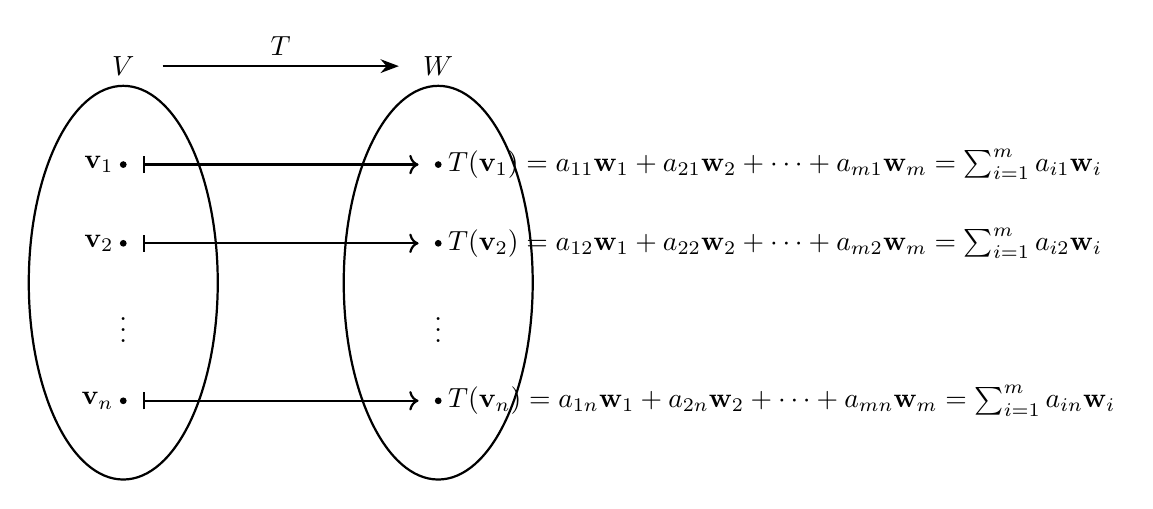
\begin{tikzpicture}
		% Draw the vector spaces V and W
		\draw[thick] (-2,0) ellipse (1.2 and 2.5); \node at (-2, 2.75) {$V$};
		\draw[thick] (2,0) ellipse (1.2 and 2.5); \node at (2, 2.75) {$W$};
		
		% Draw the arrows representing the function
		\draw[-Stealth, thick] (-1.5, 2.75) -- (1.5,2.75) node[midway, above] {$T$};
		
		\filldraw (-2,1.5) circle (1pt) node[left] {$\vec{v}_1$};
		\filldraw (2,1.5) circle (1pt) node[right] {$T(\vec{v}_1)=a_{11}\vec{w}_1+a_{21}\vec{w}_2+\cdots+a_{m1}\vec{w}_m=\sum_{i=1}^{m}a_{i1}\vec{w}_i$};
		\draw[|->, thick] (-1.75, 1.5) -- (1.75, 1.5);
		
		\filldraw (-2,.5) circle (1pt) node[left] {$\vec{v}_2$};
		\filldraw (2,.5) circle (1pt) node[right] {$T(\vec{v}_2)=a_{12}\vec{w}_1+a_{22}\vec{w}_2+\cdots+a_{m2}\vec{w}_m=\sum_{i=1}^{m}a_{i2}\vec{w}_i$};
		\draw[|->, thick] (-1.75, .5) -- (1.75, .5);
		
		\node at (-2,-.5) {$\vdots$};
		\node at (2,-.5) {$\vdots$};
		
		\filldraw (-2,-1.5) circle (1pt) node[left] {$\vec{v}_n$};
		\filldraw (2,-1.5) circle (1pt) node[right] {$T(\vec{v}_n)=a_{1n}\vec{w}_1+a_{2n}\vec{w}_2+\cdots+a_{mn}\vec{w}_m=\sum_{i=1}^{m}a_{in}\vec{w}_i$};
		\draw[|->, thick] (-1.75, -1.5) -- (1.75, -1.5);
	\end{tikzpicture}
\end{center}\vfill

\newpage
\begin{problem}
	Let $T:\mathbb{R}^2\to\mathbb{R}^2$ be the linear transformation whose standard matrix is
	\[
	A = \begin{bmatrix}
		1 & 2\\
		3 & 4
	\end{bmatrix}.
	\]
	\begin{enumerate}
		\item Compute $T\left(\begin{bmatrix}5 &6\end{bmatrix}^T\right)$.
		\item Verify that $A$ represents $T$ by checking $T(\vec{e}_1)=T\left(\begin{bmatrix}1 &0\end{bmatrix}^T\right)$ and $T(\vec{e}_2)=T\left(\begin{bmatrix}0 &1\end{bmatrix}^T\right)$.
	\end{enumerate}
\end{problem}
\begin{solution}\color{white}
	\begin{enumerate}
		\item Compute
		\[
		T\;\left(\begin{bmatrix}5\\6\end{bmatrix}\right)
		= A
		\begin{bmatrix}5\\6\end{bmatrix}
		= \begin{bmatrix}1&2\\3&4\end{bmatrix}
		\begin{bmatrix}5\\6\end{bmatrix}
		= \begin{bmatrix}1\cdot5 + 2\cdot6\\[6pt]3\cdot5 + 4\cdot6\end{bmatrix}
		= \begin{bmatrix}17\\39\end{bmatrix}.
		\]
		
		\item Verify that the columns of \(A\) are \(T(\vec{e}_1)\) and \(T(\vec{e}_2)\):
		\[
		\vec{e}_1 = \begin{bmatrix}1\\0\end{bmatrix},
		\quad
		T(\vec{e}_1) = A\,\vec{e}_1
		= \begin{bmatrix}1&2\\3&4\end{bmatrix}
		\begin{bmatrix}1\\0\end{bmatrix}
		= \begin{bmatrix}1\\3\end{bmatrix},
		\]
		which is the first column of \(A\), and
		\[
		\vec{e}_2 = \begin{bmatrix}0\\1\end{bmatrix},
		\quad
		T(\vec{e}_2) = A\,\vec{e}_2
		= \begin{bmatrix}1&2\\3&4\end{bmatrix}
		\begin{bmatrix}0\\1\end{bmatrix}
		= \begin{bmatrix}2\\4\end{bmatrix},
		\]
		which is the second column of \(A\).  Hence \(A=\begin{bmatrix}
			1 & 2\\
			3 & 4
		\end{bmatrix}=\begin{bmatrix}T(\vec{e}_1) & T(\vec{e}_2)\end{bmatrix}\).
	\end{enumerate}\color{black}\vfill\hfill\qed
\end{solution}

\newpage
\begin{problem}
	Let $T:\mathbb{R}^3\to\mathbb{R}^2$ be defined by
	\[
	T(x,y,z)=\bigl(x+2y - z,\;3x - y +4z\bigr).
	\]
	Find the matrix $[T]_{\mathcal{E}_3}^{\mathcal{E}_2}$ with respect to the standard bases $\mathcal{E}_3$ of $\mathbb{R}^3$ and $\mathcal{E}_2$ of $\mathbb{R}^2$.
\end{problem}
\begin{solution}\color{white}
	We compute the images of the standard basis vectors \(e_1,e_2,e_3\) of \(\mathbb{R}^3\):	
	\begin{align*}
	T(\vec{e}_1) &= T(1,0,0) = (1 + 2\cdot0 - 0,\;3\cdot1 - 0 +4\cdot0) = (1,3),\\
	T(\vec{e}_2) &= T(0,1,0) = (0 + 2\cdot1 - 0,\;3\cdot0 - 1 +4\cdot0) = (2,-1),\\	
	T(\vec{e}_3) &= T(0,0,1) = (0 + 2\cdot0 - 1,\;3\cdot0 - 0 +4\cdot1) = (-1,4).
	\end{align*}
	
	Since the columns of the matrix \([T]_{\mathcal{E}_3}^{\mathcal{E}_2}\) are \(T(e_1),T(e_2),T(e_3)\), we have
	\[
	[T]_{\mathcal{E}_3}^{\mathcal{E}_2}
	=\begin{bmatrix}
		\mid & \mid & \mid \\
		T(e_1) & T(e_2) & T(e_3) \\
		\mid & \mid & \mid
	\end{bmatrix}
	=\begin{bmatrix}
		1 & 2 & -1\\
		3 & -1 & 4
	\end{bmatrix}\in \R^{2\times 3}.
	\]
\color{black}\vfill\hfill\qed
\end{solution}

\newpage
\begin{problem}
Let $V = \{\,ax^2 + bx + c : a,b,c\in\mathbb{R}\}$ with basis 
\[
\mathcal{B}_V = \{\,1 + x,\; x - 1,\; x^2 + 2\},
\]
and $W = \Bbb R^2$ with basis 
\[
\mathcal{B}_W = \{\,\mathbf{e}_1 = (1,0),\;\mathbf{e}_2 = (1,1)\}.
\]
Suppose the matrix of $T:V\to W$ with respect to these bases is
\[
[T]_{\mathcal{B}_V}^{\mathcal{B}_W}
=
\begin{bmatrix}
	2 & -1 & 3\\
	0 & 4 & -2
\end{bmatrix}.
\]
Compute $T\!\bigl(- x^2+3x+2\bigr)$ in standard coordinates of $\Bbb R^2$.
\end{problem}
\begin{solution}\color{white}
	Let express $p(x)=-x^2+3x+2$ in the basis $\mathcal{B}_V$.  We look for scalars $c_1,c_2,c_3$ so that \[
	c_1(1+x) + c_2(x-1) + c_3(x^2+2) = 2 + 3x -x^2.
	\]
	Then, we have
	\[
	\begin{cases}
		c_1 - c_2 + 2c_3 = 2,\\
		c_1 + c_2 = 3,\\
		c_3 = -1.
	\end{cases}
	\] Thus we obtain \[
	c_1=\frac{7}{2},\quad c_2=-\frac{1}{2},\quad c_3=-1.
	\] So the coordinate vector is $[p]_{\mathcal{B}_V} =\begin{bmatrix}
		7/2\\ -1/2\\ -1
	\end{bmatrix}$.  Now
	\[
	[T(p)]_{\mathcal{B}_W}
	= [T]_{\mathcal{B}_V}^{\mathcal{B}_W}\;
	[p]_{\mathcal{B}_V}
	= 
	\begin{bmatrix}2&-1&3\\0&4&-2\end{bmatrix}
	\begin{bmatrix}7/2\\-1/2\\-1\end{bmatrix}
	= \begin{bmatrix}
		2\cdot\frac72 -1\cdot(-\tfrac12) +3\cdot(-1)\\
		0\cdot\frac72 +4\cdot(-\tfrac12) -2\cdot(-1)
	\end{bmatrix}
	= \begin{bmatrix}7 + \tfrac12 -3 \\ -2 +2\end{bmatrix}
	= \begin{bmatrix}\tfrac{9}{2}\\0\end{bmatrix}.
	\]
	Finally convert from $\mathcal{B}_W$–coordinates to standard: if $[T(p)]_{\mathcal{B}_W}=(\alpha,\beta)$ then
	\[
	T(p) = \alpha\,(1,0) + \beta\,(1,1)
	= (\alpha+\beta,\;\beta)
	= \Bigl(\tfrac92,\,0\Bigr).
	\]\color{black}\vfill\hfill\qed
\end{solution}
\newpage
\begin{problem}
Let $V = \R^{2\times 2}$ with basis
\[
\mathcal{B}_V = \set{\,\begin{bmatrix}
		1 & 0 \\ 0 & 0
	\end{bmatrix},\;\begin{bmatrix}
	0 & 1 \\ 1 & 0
\end{bmatrix},\;\begin{bmatrix}
0 & 0 \\ 0 & 1
\end{bmatrix}},
\]
and $W = \Bbb R^2$ with its standard basis.  Define
\[
T\left(\begin{bmatrix}a&b\\c&d\end{bmatrix}\right)
= \bigl(a + b,\;c - d\bigr).
\]
Find the matrix $[T]_{\mathcal{B}_V}^{\mathcal{E}_2}$.
\end{problem}
\begin{solution}\color{white}
	We apply $T$ to each basis element:
	
	\begin{itemize}
		\item $T(E_{11}) = T(\begin{bmatrix}1&0\\0&0\end{bmatrix})
		= (1+0,\;0-0) = (1,0).$
		\item $T(E_{12}+E_{21})
		= T(\begin{bmatrix}0&1\\1&0\end{bmatrix})
		= (0+1,\;1-0) = (1,1).$
		\item $T(E_{22})
		= T(\begin{bmatrix}0&0\\0&1\end{bmatrix})
		= (0+0,\;0-1) = (0,-1).$
	\end{itemize}
	
	Writing these as columns in the standard basis of $\Bbb R^2$ gives
	\[
	[T]_{\mathcal{B}_V}^{\text{std}}
	= \begin{bmatrix}
		1 & 1 & 0\\
		0 & 1 & -1
	\end{bmatrix}.
	\]\color{black}\vfill\hfill\qed
\end{solution}
\newpage
\begin{problem}
Let $V = \set{ax^3+bx^2+cx+d:a,b,c,d\in\R}$ with standard basis $\mathcal{B}_V=\{1,x,x^2,x^3\}$ and 
$W = \set{ax^2+bx+c:a,b,c\in\R}$ with basis $\mathcal{B}_W=\{1 + x,\;x^2,\;1\}$.  Define
\[
T(p(x)) = p'(x) + p(1).
\]
Find the matrix $[T]_{\mathcal{E}_4}^{\,\mathcal{B}_W}$.
\end{problem}
\begin{solution}\color{white}
	On the basis of $V$:
	\[
	p_1(x)=1\;\Rightarrow\;p_1'(x)=0,\;p_1(1)=1\;\Longrightarrow\;T(1)=1,
	\]
	\[
	p_2(x)=x\;\Rightarrow\;p_2'(x)=1,\;p_2(1)=1\;\Longrightarrow\;T(x)=1+1=2,
	\]
	\[
	p_3(x)=x^2\;\Rightarrow\;p_3'(x)=2x,\;p_3(1)=1\;\Longrightarrow\;T(x^2)=2x+1,
	\]
	\[
	p_4(x)=x^3\;\Rightarrow\;p_4'(x)=3x^2,\;p_4(1)=1\;\Longrightarrow\;T(x^3)=3x^2+1.
	\]
	Now write each $T(p_i)$ in the target basis $\{1+x,\;x^2,\;1\}$.
	\[
	T(1)=1 = (0)\,(1+x) + (0)\,x^2 + (1)\,(1).
	\]
	\[
	T(x)=2 = (0)\,(1+x) + (0)\,x^2 + (2)\,(1).
	\]
	\[
	T(x^2)=2x+1 = 2\bigl(1+x\bigr) -2\,(1) +0\,x^2
	= (2)\,(1+x) + (0)\,x^2 + (-2)\,(1).
	\]
	\[
	T(x^3)=3x^2+1 = (0)\,(1+x) + (3)\,x^2 + (1)\,(1).
	\]
	Hence the matrix is
	\[
	[T]_{\text{std}}^{\mathcal{B}_W}
	= \begin{bmatrix}
		0 & 0 & 2 & 0\\
		0 & 0 & 0 & 3\\
		1 & 2 & -2 & 1
	\end{bmatrix},
	\]
	where columns correspond to $T(1),T(x),T(x^2),T(x^3)$.
	\color{black}\vfill\hfill\qed
\end{solution}

\newpage
\begin{problem}
Choose any nonzero matrix \[
A\in\F^{m\times n}
\] and choose bases \begin{itemize}
	\item $\mathcal{B}_V$ for an $n$-dimensional vector space $V$ over a field $\F$ and
	\item $\mathcal{B}_W$ for an $m$-dimensional vector space $W$ over a field $\F$.
\end{itemize} Define the linear map $T:V\to W$ by \[
[T]_{\mathcal{B}_V}^{\mathcal{B}_W}=A.
\] \begin{enumerate}
	\item Pick a vector $\vec{v}\in V$ (in coordinates relative to $\mathcal{B}_V$) and compute $T(\vec{v})$ in the coordinates of $W$.
	\item Determine $\ker T$, $\mathrm{im} T$, and $\mathrm{rank} T$.
\end{enumerate}
\end{problem}
\begin{solution}
\ \vfill\hfill\qed
\end{solution}

\newpage
\adjustbox{scale=2, center}{
	\begin{tikzcd}
	V \arrow[rrrr, "\phi_n=\mathrm{Id}_n", shift left=0] \arrow[dddd, "T"'] \arrow[blue, dddd, shift left=3]                
	&  &  &  & \F^n \arrow[red, dddd, "A=\phi_m\circ T\circ \phi_n^{-1}"'] \arrow[blue, llll, "\phi_n^{-1}=\mathrm{Id}_n", shift left=2]                 \\
	&  &  &  &                                                          \\
	&  &  &  &                                                          \\
	&  &  &  &                                                          \\
	W \arrow[rrrr, "\phi_m=\mathrm{Id}_m"] \arrow[blue, rrrr, shift left=3] &  &  &  & \mathbb{F}^m 
	%\arrow[uuuu, "\Phi_m^{-1}"', shift right=3]
\end{tikzcd}}

\end{document}